\documentclass[english,floatsintext,man]{apa6}

\usepackage{amssymb,amsmath}
\usepackage{ifxetex,ifluatex}
\usepackage{fixltx2e} % provides \textsubscript
\ifnum 0\ifxetex 1\fi\ifluatex 1\fi=0 % if pdftex
  \usepackage[T1]{fontenc}
  \usepackage[utf8]{inputenc}
\else % if luatex or xelatex
  \ifxetex
    \usepackage{mathspec}
    \usepackage{xltxtra,xunicode}
  \else
    \usepackage{fontspec}
  \fi
  \defaultfontfeatures{Mapping=tex-text,Scale=MatchLowercase}
  \newcommand{\euro}{€}
\fi
% use upquote if available, for straight quotes in verbatim environments
\IfFileExists{upquote.sty}{\usepackage{upquote}}{}
% use microtype if available
\IfFileExists{microtype.sty}{\usepackage{microtype}}{}

% Table formatting
\usepackage{longtable, booktabs}
\usepackage{lscape}
% \usepackage[counterclockwise]{rotating}   % Landscape page setup for large tables
\usepackage{multirow}		% Table styling
\usepackage{tabularx}		% Control Column width
\usepackage[flushleft]{threeparttable}	% Allows for three part tables with a specified notes section
\usepackage{threeparttablex}            % Lets threeparttable work with longtable

% Create new environments so endfloat can handle them
% \newenvironment{ltable}
%   {\begin{landscape}\begin{center}\begin{threeparttable}}
%   {\end{threeparttable}\end{center}\end{landscape}}

\newenvironment{lltable}
  {\begin{landscape}\begin{center}\begin{ThreePartTable}}
  {\end{ThreePartTable}\end{center}\end{landscape}}




% The following enables adjusting longtable caption width to table width
% Solution found at http://golatex.de/longtable-mit-caption-so-breit-wie-die-tabelle-t15767.html
\makeatletter
\newcommand\LastLTentrywidth{1em}
\newlength\longtablewidth
\setlength{\longtablewidth}{1in}
\newcommand\getlongtablewidth{%
 \begingroup
  \ifcsname LT@\roman{LT@tables}\endcsname
  \global\longtablewidth=0pt
  \renewcommand\LT@entry[2]{\global\advance\longtablewidth by ##2\relax\gdef\LastLTentrywidth{##2}}%
  \@nameuse{LT@\roman{LT@tables}}%
  \fi
\endgroup}


  \usepackage{graphicx}
  \makeatletter
  \def\maxwidth{\ifdim\Gin@nat@width>\linewidth\linewidth\else\Gin@nat@width\fi}
  \def\maxheight{\ifdim\Gin@nat@height>\textheight\textheight\else\Gin@nat@height\fi}
  \makeatother
  % Scale images if necessary, so that they will not overflow the page
  % margins by default, and it is still possible to overwrite the defaults
  % using explicit options in \includegraphics[width, height, ...]{}
  \setkeys{Gin}{width=\maxwidth,height=\maxheight,keepaspectratio}
\ifxetex
  \usepackage[setpagesize=false, % page size defined by xetex
              unicode=false, % unicode breaks when used with xetex
              xetex]{hyperref}
\else
  \usepackage[unicode=true]{hyperref}
\fi
\hypersetup{breaklinks=true,
            pdfauthor={},
            pdftitle={A thorough evaluation of the Language Environment Analysis (LENATM) system},
            colorlinks=true,
            citecolor=blue,
            urlcolor=blue,
            linkcolor=black,
            pdfborder={0 0 0}}
\urlstyle{same}  % don't use monospace font for urls

\setlength{\parindent}{0pt}
%\setlength{\parskip}{0pt plus 0pt minus 0pt}

\setlength{\emergencystretch}{3em}  % prevent overfull lines

\ifxetex
  \usepackage{polyglossia}
  \setmainlanguage{}
\else
  \usepackage[english]{babel}
\fi

% Manuscript styling
\captionsetup{font=singlespacing,justification=justified}
\usepackage{csquotes}
\usepackage{upgreek}



\usepackage{tikz} % Variable definition to generate author note

% fix for \tightlist problem in pandoc 1.14
\providecommand{\tightlist}{%
  \setlength{\itemsep}{0pt}\setlength{\parskip}{0pt}}

% Essential manuscript parts
  \title{A thorough evaluation of the Language Environment Analysis (LENATM)
system}

  \shorttitle{IN PREP - LENA EVAL}


  \author{many\textsuperscript{1}}

  % \def\affdep{{""}}%
  % \def\affcity{{""}}%

  \affiliation{
    \vspace{0.5cm}
          \textsuperscript{1}   }

  \authornote{
    Correspondence concerning this article should be addressed to many, .
    E-mail:
  }


  \abstract{waiting}
  




\begin{document}

\maketitle

\setcounter{secnumdepth}{0}



\subsubsection{Brief introduction to LENA(R)
products}\label{brief-introduction-to-lenar-products}

\subsubsection{Previous validation work}\label{previous-validation-work}

\subsubsection{Present work}\label{present-work}

\subsection{Methods}\label{methods}

\subsubsection{Corpora}\label{corpora}

The data for the evaluation comes from two different projects. The
largest one is the ACLEW project (Bergelson et al., 2017b Databrary
volume; Soderstrom et al AMPPS under review); in this paper we focus on
four different corpora of child daylong recordings that have been pooled
together, sampled, and annotated in a coordinated manner. These four
corpora are: the Bergelson corpus (\enquote{BER}) from US English
families from the upstate New York area (Bergelson, 2016), the LuCiD
Language 0--5 corpus (\enquote{L05}) consisting of English-speaking
families from Northwest England (Rowland et al., 2018), the McDivitt and
Winnipeg corpora ( \enquote{MCD}) of Canadian English families (McDivitt
\& Soderstrom, 2016), and the Warlaumont corpus (\enquote{WAR}) of US
English from Merced, California (Warlaumont et al., 2016). Some
recordings in BER, and all recordings in MCD and WAR are available from
HomeBank repository (VanDam et al., 2016). The second project contains a
single corpus collected from Tsimane' speaking families in Bolivia
(Scaff et al., in prep.; here \enquote{TSI}).

Key properties of the five corpora are summarized in Table 2. Each
corpus consists of daylong (4--16 hour) at-home recordings; each corpus
samples from a unique community. Corpora span languages and dialects;
socioeconomic environment varying both within and across corpora. In
each recording, the key child (\enquote{participant}) wears a LENA
recorder in a special vest throughout a normal day.

For the four ACLEW corpora, out of the 106 recorded participants,
daylong recordings from 10 infants from each corpus were chosen for
manual annotation, selected to represent a diversity of ages (0--36
months) and socio-economic contexts. In the SOD corpus, sensitive
information was found in one of the files, and thus one child needed to
be excluded. The tenth day for this corpus was a second day by one of
the 9 included children. From each daylong file, fifteen 2-minute
non-overlapping audio (with a 5-minute context window) were randomly
sampled from the entire daylong timeline for manual annotation. This 30
minute sample corresponded to approximately 1 minute of annotated speech
per key child (collapsing across all speaker categories).

The TSI corpus consisted of 1-2 daylong recordings from 12 infants, out
of the 25 recorded from field work that year; the other 13 had been
recorded using other devices (not the LENA DLP). From these daylong
files, 1-minute segments were sampled in a period fashion. That is, for
each day, we skipped the first 33 minutes to allow the family to
acclimate to the recorder, and then extracted 1 minute (with a 5-minute
context window) every 60 minutes, until the end of the recording was
reached. This resulted in 4 to 16 minutes of manually annotated audio
per child per recording (mean = 12.64 minutes), and an average of 3
minutes of speech per key child (collapsing across all speaker
categories).

We chose to sample 1 or 2 minutes at a time (Tsimane, and ACLEW corpora,
respectively) because conversations are likely to be bursty (Goh \&
Barbasi; cf.~Slone et al Fausey et al ICIS18 session). That is, it is
likely the case that speech is not produced at a periodic rate (e.g.,
one phrase every 20 seconds), but rather it occurs in bursts (a
conversation is followed by a long period of silence between the
conversational partners, followed by another bout of conversation,
perhaps with different interlocutors, followed by silence, and so on).
In this context, imagine that you sample a 5-second stretch. If you find
speech in that stretch, then it is likely you have by chance fallen on a
conversation bout; if you do not find speech, then you have likely found
a silence bout. If you were to extend that selection out to several
minutes, then it is likely that you will simply add more material from
the same type (i.e.~conversation bout or silence bout). As a result, any
sampling method that favors medium-sized stretches (5-15 minutes) will
tend to end up with samples that are internally homogeneous (throughout
the 5 minutes, there is a conversation), but highly heterogeneous as a
collection if sampling is random throughout the day. This in turn would
lead to artificially high correlations between LENA and human metrics in
all dependent variables (e.g., since probably little speech, fewer
turns, and fewer child vocalizations will be found in silent bouts and
more in conversational ones). Thus, our strategy of sampling
randomly/periodically and in short stretches is more likely to represent
both conversational and short bouts, and to capture finer-grained
variation in speech quantity.

In the 5 corpora, the 1- or 2-min samples were annotated for all
hearable utterance boundaries and talker ID. In ACLEW corpora
\footnote{see Casillas et al., 2017a, 2017b for the general annotation protocol, and Soderstrom et al., submitted to AMPPS, for an introduction to the databases},
talker IDs reflected unique individual talkers, but were coded in such a
way to readily allow mapping onto LENAs talker categories (e.g.~key
child, other children, female adult, male adult). In the TSI corpus,
only the key child and one female adult whose voice recurred throughout
the day were individually identified, with all other talkers being
classified on the basis of broad age and sex into male adult, female
adult, and other children. The ACLEW datasets had other coding levels
which will not be discussed here.

\subsubsection{Processing}\label{processing}

Several different time units are needed to clarify how different metrics
are calculated (see Figure XX). Clips refer to the 1- or 2-minute
samples extracted from recordings. This is the basic unit at which child
vocalization counts and conversational turn counts can be established.
In addition, since most previous work evaluating adult word counts did
so at the clip level, we do so here as well.

\begin{figure}
\centering
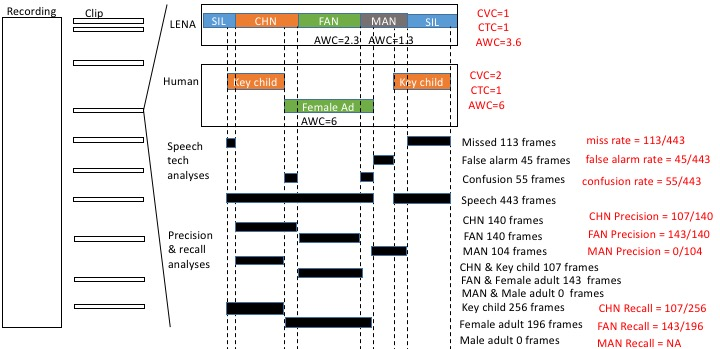
\includegraphics{fig_levels.jpg}
\caption{Levels at which performance is evaluated.}
\end{figure}

The other metrics require a more detailed explanation, conveyed
graphically in Figure XX. The stretch of time that has been assigned to
a speech or non-speech category by LENA is a segment. In one clip, there
may be just one long segment (e.g., the whole clip has been assigned to
Silence by LENA); or there may be more (e.g., the first 5 seconds are
attributed to the key child, then there is a 50-second Silence segment,
and the final 5 seconds are attributed to a Female Adult). In LENA's
automated analysis, only one of these categories may be active at a
given point in time. In contrast, we typically speak of utterances or
vocalizations to refer to stretches of speech detected by humans and
assigned to different talkers. Again, clips may have zero or more
utterances. Unlike LENA, however, a given point in time may be
associated with multiple speakers. Given that there need not be a
one-to-one correspondence between LENA segments and human utterances, we
need to define smaller time units that can be used to check for
agreement. In this paper, we use 10 ms frames. This is the basic time
unit used for all classification accuracy estimations, which are
introduced in more detail in the next subsection.

\subsubsection{LENA classification
accuracy}\label{lena-classification-accuracy}

Our first goal was to establish LENA talker tag accuracy, particularly
for the four broad LENA talker categories (key child, other child,
female adult, male adult; or CHN, CXN, FAN, MAN), but taking into
account other categories (with some limitation on their interpretation).
We calculated accuracy in two complementary ways. First, we used three
frame-based, standard metrics of speech and talker segmentation to allow
direct comparison with other systems in the speech technology literature
(False Alarms, Misses, Confusion Rate). We also use Diarization Error
Rate, which is derived from the first three metrics; together these
provide a stringent and standard test of accuracy. Second, we used
frame-based precision and recall of each category to provide an
intuitive representation of the error patterns shown by this system. In
both cases, electronic voices were rare in the ACLEW annotations and not
coded at all (by design) in the Tsimane data, they were mapped onto
silence.

\paragraph{Speech and talker segmentation
metrics}\label{speech-and-talker-segmentation-metrics}

The original coding was converted using custom-written python scripts
into rttm format (REF), a text-based format indicating, for each
vocalization, its start time, duration, and speaker. This representation
was used in pyannote.metrics (REF) to compute four standard diarization
metrics: rate of false alarm for speech, rate of misses for speech, rate
of confusion between talkers, and the derived diarization error rate
(DER). These are calculated with the following formulas at the level of
each clip, where FA (false alarm) is the number of frames during which
there is no talk according to the human annotator but during which LENA
found some talk; M (miss) is the number of frames during which there is
talk according to the human annotator but during which LENA found no
talk; C (confusion) is the number of frames correctly classified as LENA
as containing talk, but whose voice type has not been correctly
identified (when the LENA model recognizes female adult speech where
there is male adult speech for instance), and T is the total number of
frames that contain talk according to the human annotation:

\begin{itemize}
\tightlist
\item
  false alarm rate = FA/T,
\item
  miss rate = M/T,
\item
  confusion rate = C/T,
\item
  DER = (FA+M+C)/T,
\end{itemize}

In the human annotation, there is no class representing overlapping
speech as such. For the sake of completeness and full comparison with
the LENA model, time where two or more different speech sources were
active at the same time, according to the human annotators, have been
mapped to the class \enquote{overlap} post hoc. This allows us to
compare this Overlap class to LENA's OLN (and, for the precision/recall
analysis introduced next, OLF) by the LENA model. Therefore, the
confusion rate is computed based on the matches in Table XX.

Table XX: Correspondances between LENA and our human annotation.
*Electronic voices were only annotated in the ACLEW dataset. Although
some Tsimane' families listen to the radio, radio speech was not
annotated in the TSI corpus.

Please remember that the overlap category is not defined the same way as
the LENA overlap category. For LENA, overlap between any two categories
falls within overlap -- i.e., CHN+TV would be counted towards overlap as
would FAN+FAN; whereas for us, only overlap between two talker
categories (e.g., key child and female adult) counts as overlap.
Similarly, the TVN is not equivalent to the electronic speech tag in the
ACLEW coding.

\paragraph{Precision and recall}\label{precision-and-recall}

This evaluation looks in more detail at the pattern of errors, by
assessing how LENA and human annotators agreed and disagreed. In both
precision and recall, the numerator is the intersection between a LENA
tag and a human tag (e.g., the number of frames that LENA classified as
CHN and the annotator classified as Key child; notice, there is no
constraint that these two categories by conceptually the same). The
denominator differs: To calculate precision, we divide that number by
the total number of frames attributed to a category by LENA, whereas for
recall, we divide by the total number of frames attributed to a category
by the human annotator.

\subsubsection{CVC and CTC evaluation}\label{cvc-and-ctc-evaluation}

From the human annotation, each vocalization by the key child counted
towards the total Child Vocalization Count (CVC) for a given clip. For
the Conversational Turn Count (CTC), a sequence of key child and any
adult (or vice versa) within 5 seconds counted towards the clip total
CTC.

\subsubsection{AWC evaluation}\label{awc-evaluation}

For the AWC portion of this evaluation, we could only use transcriptions
from the four ACLEW corpora, since the TSI corpus has not been
transcribed (and thus lacks word counts). In contrast, annotators for
the four ACLEW corpora were proficient in the language spoken in the
daylong recording, and transcribed all adult speech based using
canonical lexical forms (e.g. \enquote{wanna}, not \enquote{want to}) in
keeping with minCHAT format (MacWhinney).

Reference adult word counts were determined by counting all
unambiguously transcribed words spoken by adult talkers. This was
achieved by first discarding all non-lexical transcript entries such as
non-linguistic communicative sounds, paralinguistic markers, and markers
indicating incomprehensible speech. In addition, all utterances from the
key child and other children were omitted from the Adult Word Count. The
remaining orthographic entries separated by whitespaces were then
counted as gold standard target words for LENA to detect.

As for LENA word counts, the regions sampled for manual annotation were
not guaranteed to perfectly align with LENA utterances. Of all LENA
utterances overlapping with the annotated speech, 14\% had only partial
overlap with the annotations. To match LENA AWCs with the annotated word
counts, words from the partially overlapping LENA utterances were
included in proportion to the amount of overlap between the LENA turn
and the reference segment in question (e.g., if 10\% of a LENA-estimated
utterance was overlapping with a manually-annotated utterance, 10\% of
the total LENA AWC estimate for the given turn was included in the LENA
word count estimate for that reference segment).

\subsection{Results}\label{results}

Before starting, we provide some general observations based on the human
annotation. Silence is extremely common, constituting 79\% of the
frames. In fact, 45\% of clips contained no speech by any of the human
speaker types (according to the human annotators). As for speakers,
female adults make up 11\% of the frames, the child contributes to 4\%
of the frames, whereas male adult voices, other child voices, and
electronic voices are found in only 1\% of the frames each. Overlap
makes up the remaining 3\% of the frames. The following consequences
ensue: if frame-based accuracy is sought, a system that classifies every
frame as silence would be 79\% correct. This is of course not what we
want, but it indicates that systems adapted to this kind of speech
should tend to have low \enquote{false alarm} rates, i.e.~a preference
for being very conservative as to when there is speech. If the system
does say there is speech, then it had better say that this speech comes
from female adults, who provide a great majority of the speech. In
second place, it should be key child. Given that male adults and other
children are rare, a system that makes a lot of mistakes in these
categories may still have a good global performance, because these
categories are extremely rare.

\subsubsection{LENA classification accuracy: False alarms, misses,
confusion}\label{lena-classification-accuracy-false-alarms-misses-confusion}

Our first analysis is based on standard speech technology metrics, which
put errors in the perspective of how much speech there is. That is, if
10 frames are wrong in a file where there are 100 frames with speech,
this is a much smaller problem than if 10 frames are wrong in a file
where there is 1 frame with speech. In other words, these metrics should
be considered relative error metrics. One problem, however, emerges when
there is no speech whatsoever in a given file. In the speech technology
literature, this is never discussed, because most researchers working on
this are basing their analyses on files that have been selected to
contain speech (e.g., recorded in a meeting, or during a phone
conversation). We still wanted to take into account clips with no speech
inside because it is key for our research goals: We need systems that
can deal well with long stretches of silence, because we want to measure
how much speech children hear. Indeed, as mentioned above, 45\% of our
clips had no speech whatsoever. In these cases, the false alarm, miss,
and confusion rates are all undefined, because the denominator is zero.
In all likelihood, this leads to an overestimation of LENA's
performance, because potential false alarms in these files are not
counted against the system. It also occurred that there was just a
little speech; in this case, the denominator is very small, and
therefore the ratio for these two metrics ended up being a very large
number. To avoid such outliers having an undue impact on our report, we
present medians (rather than means).

There were, a priori, several ways of analyzing the data:

\begin{itemize}
\tightlist
\item
  collapsing near and far together (i.e., CHN and CHF were mapped onto a
  single CH category)
\item
  treating the near and far categories separately (i.e., CHN and CHF are
  both treated as \enquote{speakers}, but not the same one)
\item
  not considering TV as a speaker category, since it is conceptually not
  identical to the electronic voices detected by ACLEW human annotators;
  in this case, the gold annotations should also map electronic voices
  to non-speech or silence
\item
  not considering OLN as a speaker category, since it is not
  conceptually identical to the overlap derived from humans' annotating
  different speaker categories.
\end{itemize}

We thought the most informative decision would be to report on several
of these settings, albeit briefly. We start with the situation that
yields the best LENA performance: Electronic voices in the gold
annotation are mapped onto silence, so that the categories found in the
human annotation are FEM, MAL, CHI, OCH, and overlap; in the LENA
annotation, only CHN, FAN, MAN, and CXN are considered speakers (with
all far categories, TVN, and OLN all mapped onto silence). In this
setting, LENA's false alarm (i.e., saying that someone was speaking when
they were not) had a median of 12\%, whereas the miss rate had a median
of 49\%. The confusion rate, as mentioned above, is only calculated for
the correctly detected speech (i.e., not the speech that was missed,
which counts towards the miss rate, nor the speech that was falsely
identified, which is considered in the false alarm). The confusion rate
was very low, with a median of 10\%. These three metrics can be added
together into a single \enquote{diarization error rate}. The median
diarization error rate over the clips that had some speech was 79\%.

If electronic voices in the gold annotation are still mapped onto
silence and in the LENA annotation, CHN, FAN, MAN, CXN as well as OLN
are considered speakers (with all far categories as well as TVN mapped
onto silence), so that the human categories considered were CHI, FEM,
MAL, OCH, and overlap; and the LENA categories considered were CHN, FAN,
MAN, CXN, and OLN. In this setting, LENA's false alarm, missed, and
confusion rate medians were 33\%, 21\%, and 28\% respectively, for a
total median diarization error of 82\%. Performance likely degrades
because OLN is not picking up the same regions as the overlapping speech
found in the human annotations.

Next, we allowed the electronic voices segmented by humans, and TVN
among the LENA speaker categories, to be considered during the
evaluation (rather than mapping them all to non-speech or silence), so
that the human categories considered were CHI, FEM, MAL, OCH, overlap,
and electronic; and the LENA categories considered were CHN, FAN, MAN,
CXN, OLN, and TVN. LENA's false alarm, missed, and confusion rate
medians were 40\%, 18\%, and 30\% respectively, for a total median
diarization error of 88\%. Performance likely degrades because TVN is
not picking up the electronic speech segmented by ACLEW annotators.

Finally, we declared the maximum possible number of categories: The
human categories considered were still CHI, FEM, MAL, OCH, overlap, and
electronic; but the LENA categories considered were CHN, FAN, MAN, CXN,
OLN, TVN, CHF, FAF, MAF, CXF, OLF, TVF. LENA's false alarm, missed, and
confusion rate medians were 74\%, 7\%, and 41\% respectively, for a
total median diarization error of 122\%. Performance degrades because
everything is treated as speech, leading to huge apparent false alarm
rates.

\subsubsection{LENA classification accuracy: Precision and
recall}\label{lena-classification-accuracy-precision-and-recall}

By now, we have established that the best performance (when
\enquote{far} labels such as CHF and OLF are mapped onto silence, as are
TVN and OLN), the overall relative diarization error rate is about 79\%,
due mainly to missing speech (49\%), with false alarms (12\%) and
confusion between talker categories (10\%) constituting a relatively
small proportion of errors. However, this metric may not capture what
our readers are interested in, for two reasons. First, this metric gives
more importance to correctly classifying segments as speech versus
non-speech (False alarms + misses) than confusing talkers (confusion).
Second, many LENA adopters use the system not to make decisions on the
sections labeled as non-speech, but rather on sections labeled as
speech, and particularly those labeled adults and key child. The metrics
above do not give more importance to these two categories, and do not
give us insight on the patterns of error made by the system. Looking at
precision of speech categories is crucial for users who interpret LENA's
estimated quantity of adult speech or key child speech, as low precision
means that some of what LENA called e.g.~key child was not in fact the
key child, and thus it is providing overestimates. Looking at recall may
be most interesting for adopters who intend to employ LENA as a
first-pass annotation: the lower the recall, the more is missed by the
system and thus cannot be retrieved (because the system labeled it as
something else, which will not be inspected given the original filter).
Recall also impacts quantity estimates, since it indicates how much was
missed of that category.

Therefore, this subsection shows confusion matrices, containing
information on precision and recall, for each key category. For this
analysis, we collapsed over all human annotations that contained overlap
between two speakers into a category called \enquote{overlap}. Please
remember that this category is not defined the same way as the LENA
overlap category. For LENA, overlap between any two categories falls
within overlap -- i.e., CHN+TV would be counted towards overlap; whereas
for us, only overlap between two talker categories (e.g., key child and
female adult) counts as overlap.

\begin{figure}
\centering
\includegraphics{main_document_files/figure-latex/ggprec-1.pdf}
\caption{}
\end{figure}

We start by explaining how to interpret one cell in Figure (precision):
Focus on the crossing of the human category FEM and the LENA category
FAN; when LENA tags a given frame as FAN, this corresponds to a frame
tagged as being a female adult by the human 52\% of the time. This
category, as mentioned above, is the most common speaker category in the
audio, so that over 57k frames (representing 52\% of the frames tagged
as FAN by LENA) were tagged as being female adult by both the human and
LENA. The remaining 2, 0, 1, 8, 0, and 37\% of frames that LENA tagged
as FAN were actually other categories according to our human coders:
37\% were silence, 8\% were in regions of overlap between speakers or
between a speaker and an electronic voice, and 3\% were due to
confusions with other speaker tags. Inspection of the rest of the
confusion matrix shows that, other than silence, this is the most
precise LENA tag.

Precision for CHN comes in secondplace, at 39\%; thus, fewer than half
of the frames labeled as being the key child are, in fact, the key
child. The majority of the frames, LENA incorrectly tagged as being the
key child are actually silence (or rather, lack of speech) according to
the human annotator (44\%), with the remaining errors being due to
confusion with other categories: About 8\% of them are actually a female
adult; 2\% are another child; and 7\% are regions of overlap across
speakers, according to our human coders.

MAN and CXN score similarly, 8 and 6\% respectively, meaning that less
than a tenth of the areas LENA tagged as being these speakers actually
correspond to them. As with the key child, most errors are due to LENA
tagging silent frames as these categories. However, in this case
confusion with other speaker tags is far from negligible. In fact, the
most common speaker tag in the human annotation among the regions that
LENA tagged as being MAN were actually female adult speech (27\%); and,
for CXN, it was not uncommon to find a CXN tag for a frame human
listeners identified as a female adult (17\%) or the key child (6\%). In
a nutshell, this suggests extreme caution before undertaking any
analyses that rely on the precision of MAN and CXN, since most of what
is being tagged as such is silence or other speakers.

Another observation is that the \enquote{far} tags of the speaker
categories do tend to more frequently correspond to what humans tagged
as silence (74\%) than the \enquote{near} tags (54\%), and thus it is
reasonable to exclude them from consideration. The relatively high
proportion of near LENA tags that correspond to regions that humans
labeled as silence could be partially due to the fact that the LENA
system, in order to process a daylong recording quickly, does not make
judgments on small frames independently, but rather imposes a minimum
duration for all speaker categories, padding with silence in order to
achieve it. Thus, any key child utterance that is shorter than .6 secs
will contain as much silence as needed to achieve this minimum (and more
for the other talker categories). Our system of annotation, whereby
human annotators had no access whatsoever to the LENA tags, puts us in
an ideal situation to assess the impact of this design decision, because
any annotation that starts from the LENA segmentation should bias the
human annotator to ignore such short interstitial silences to a greater
extent than if they have no access to their tags whatsoever.

These analyses shed light on the extent to which we can trust the LENA
tags to contain what the name indicates. We now move on to recall, which
indicates a complementary perspective: how much of the original
annotations were captured by LENA.

\begin{figure}
\centering
\includegraphics{main_document_files/figure-latex/ggrec-1.pdf}
\caption{}
\end{figure}

Again, we start with an example to facilitate the interpretation of this
figure: The best performance for a talker category this time is CHN:
Nearly half of the original frames humans tagged as being uttered by the
key child were captured by the LENA under the CHN tag. Among the
remaining regions that humans labeled as being the key child, 22\% was
captured by LENA's CXN category and 20\% by its OLN tag, with the
remainder spread out across several categories. This result can be taken
to suggest that an analysis pipeline that uses the LENA system to
capture the key child's vocalizations by extracting only CHN regions
will get nearly half of the key child's speech. Where additional human
vetting is occuring in the pipeline, such researchers may consider
additionally pulling out segments labeled as CXN, since this category
actually contains a further 22\% of the key child's speech. Moreover, as
we saw above, over a third of these LENA tags corresponds to the key
child, which means that human coders who are re-coding these regions
could filter out the two thirds that do not.

Many colleagues also use the LENA as a first pass to capture female
adult speech via their FAN label. Only 30 of the female adult speech can
be captured this way. Unlike the case of the key child, missed female
speech is classified into many of the other categories, and thus there
may not exist an easy solution (i.e., one would have to pull out all
examples of many other categories to get at least half of the original
female adult). However, if the hope is to capture as much of the female
speech as possible, perhaps a solution may be to also pull out OLN
regions, since these capture a further 25\% of the original female adult
speech and, out of the OLN tags, 16\% are indeed female adults (meaning
that human annotators re-coding these regions need to filter out 4 out
of 5 clips, on average).

For the remaining two near speaker labels (MAN, CXN), recall averaged
15\%, meaning that less than a quarter of male adult and other child
speech is being captured by LENA. In fact, most of these speakers'
contributions are being tagged by the LENA as OLN (mean across MAN and
CXN 34\%) or silence (mean across MAN and CXN 7\%), although the
remaining sizable proportion of misses is actually distributed across
many categories.

Finally, as with precision, the \enquote{far} categories show worse
performance than the \enquote{near} ones. It is always the case that a
higher percentage of frames is \enquote{captured} by the near rather
than the far labels. For instance, out of all frames attributed to the
key child by the human annotator, 42\% were picked up by the LENA CHN
label versus 0\% by the LENA CHF label. This result can be used to argue
why, when sampling LENA daylong files using the LENA software, users
need not take into account the \enquote{F} categories.

\subsubsection{Child Vocalization Counts (CVC)
accuracy}\label{child-vocalization-counts-cvc-accuracy}

Given the inaccuracy of far LENA tags, and in order to follow the LENA
system procedure, we only counted vocalizations attributed to CHN and
ignored those attributed to CHF. As shown in Figure (CVC), there is a
strong association between clip-level counts estimated via the LENA
system and those found in the human annotations: the Pearson correlation
between the two was r = 0.71 (p = 0.00) when all clips were taken into
account, and r = 0.77 (p = 0.00) when only clips with some child speech
(i.e., excluding clips with 0 counts in both LENA and human annotations)
were considered. This suggests that the LENA system captures differences
in terms of number of child vocalizations across clips well.

\begin{figure}
\centering
\includegraphics{main_document_files/figure-latex/cvc-fig-1.pdf}
\caption{}
\end{figure}

However, users need more: They also interpret the absolute number of
vocalizations found by LENA. Therefore, it is important to also bear in
mind the absolute error rate and the relative error rate. The absolute
error rate tells us, given a LENA estimate, how close the actual number
may be. The relative error rate puts this number in relation to the
actual number of vocalizations tagged by the human coder. For instance,
imagine that we find that LENA errs by 10 vocalizations according to the
absolute error rate; this means that, on average across short clips like
the ones used here, the numbers by LENA would be off by 10
vocalizations. We may think this number is small; by using the relative
error rate, we can check whether it is small relative to the actual
number: An error of 10 vocalizations would seem less problematic if
there are 100 vocalizations on average (LENA would be just 10\% off)
than if there are 10 (LENA would be doubling the number of
vocalizations).

The absolute error rate ranged from -47 to 30, with a mean of -1.63 and
a median of 0. Since these numbers can be affected by silent clips, in
which both humans and LENA agree on there not being any vocalizations,
we also calculated the absolute error rate excluding these clips. In
this case, the absolute error rate ranged from -47 to 13, with a mean of
-5.35 and a median of -4. As for relative error rates, these require the
number in the denominator to be non-null. For this analysis, therefore,
we need to remove the 460 clips in which the human annotator said there
were no child vocalizations whatsoever. When we do this, the mean
relative error rate ranged from -100 to 800, with a mean of -20.17 and a
median of -44.44

\subsubsection{Conversational Turn Counts (CTC)
accuracy}\label{conversational-turn-counts-ctc-accuracy}

\begin{figure}
\centering
\includegraphics{main_document_files/figure-latex/ctc-fig-1.pdf}
\caption{}
\end{figure}

Again, we only considered \enquote{near} speaker categories in the turn
count, and applied the same rule the LENA does, where a turn can be from
the key child to an adult or vice versa, and should happen within 5
seconds to be counted. The association between clip-level LENA and human
CTC was weaker than that found for CVC: the Pearson correlation between
the two was r = 0.55 (p = 0.00) when all clips were taken into account,
and r = 0.47 (p = 0.00) when only clips with some child speech (i.e.,
excluding 322 clips with 0 counts in both LENA and human annotations)
were considered. The absolute error rate ranged from -75 to 25, with a
mean of -6.82 and a median of 0. The absolute error rate excluding clips
where both human and LENA counts were zero ranged from -75 to 20, with a
mean of -15.67 and a median of -12. As for relative error rates, these
require the number in the denominator to be non-null. For this analysis,
therefore, we need to remove the 427 clips in which the human annotator
said there were no child-adult or adult-child turns whatsoever. When we
do this, the mean relative error rate ranged from -100 to 366.67, with a
mean of -64.64 and a median of -81.82

\subsubsection{Adult Word Counts
accuracy}\label{adult-word-counts-accuracy}

\begin{figure}
\centering
\includegraphics{main_document_files/figure-latex/awc-fig-1.pdf}
\caption{}
\end{figure}

One child in the SOD corpus was learning French. We have included this
child to increase power, but results without this one child are nearly
identical. The association between clip-level LENA and human AWC was
strong: the Pearson correlation between the two was r=0.75 (p=0.00) when
all clips were taken into account, and r=0.69 (p=0.00) when only clips
with some child speech (i.e., excluding 309 clips with 0 counts in both
LENA and human annotations) were considered. This suggests that the LENA
system captures differences in terms of number of child vocalizations
across clips well. The absolute error rate ranged from -211 to 157, with
a mean of -0.20 and a median of 0. The absolute error rate excluding
clips where both human and LENA counts were zero ranged from -211 to
157, with a mean of 0.46 and a median of -2. As for relative error
rates, these require the number in the denominator to be non-null. For
this analysis, therefore, we need to remove the 361 clips in which the
human annotator said there were no child-adult or adult-child turns
whatsoever. When we do this, the mean relative error rate ranged from
-100 to 7400, with a mean of 55.04 and a median of -17.78

\subsubsection{Effects of age and differences across
corpora}\label{effects-of-age-and-differences-across-corpora}

The preceding sections include results that are wholesale, over all
corpora. However, we have reason to believe that performance could be
higher for the corpora collected in North America (BER, WAR, SOD) than
those collected in other English-speaking countries (L05) or non-English
speaking populations (TSI). Additionally, our age ranges are wide, and
in the case of TSI children, some of the children are older than the
oldest children in the LENA training set. To assess whether accuracy
varies as a function of corpora and child age, we fit mixed models as
follows.

We predicted false alarm, miss, and confusion rates (when all
\enquote{F} categories, TV, and overlap were mapped onto silence, which
yielded the best results in Section XX) from corpus, child age, and the
interaction as fixed effects, child ID as random effect, on clips where
there was some speech according to the human annotator. We followed up
with an Analysis of Variance (type 2) to assess significance. In none of
these analyses was corpus, child age, or their interaction significant.

For CVC, we fit a mixed model where CVC according to the human was
predicted from CVC according to LENA, in interaction with corpus and
age, as fixed factors; with child ID as random effect. An Analysis of
Variance (type 2) found a triple interaction, suggesting that the
predicted value of LENA with respect to human CVC depended on both the
corpus and the child age; and a two-way interaction between CVC by LENA
and corpus. To investigate these further, we fit a model where CVC
according to the human was predicted from CVC according to LENA in
interaction with age (as fixed factors, with child ID as random) within
each corpus separately. This revealed a significant interaction between
LENA CVC and age for BER (indicating that the predictive value of LENA
CVC increased with child age), whereas for the other four corpora this
interaction was not significant, nor was the main effect of age, and
only the LENA CVC emerged as a significant predictor of variance in
child vocalization counts derived from human
annotation.\href{For\%20both\%20BER\%20and\%20WAR,\%20the\%20variance\%20associated\%20to\%20the\%20child\%20ID\%20random\%20factor\%20was\%20zero.\%20This\%20suggests\%20a\%20mixed\%20model\%20was\%20not\%20necessary,\%20as\%20child\%20ID\%20is\%20not\%20explaining\%20any\%20additional\%20variance,\%20but\%20it\%20does\%20not\%20alter\%20the\%20interpretation\%20in\%20the\%20main\%20text.}{1}

For CTC, we fit a mixed model where CTC according to the human was
predicted from CTC according to LENA, in interaction with corpus and
age, as fixed factors; with child ID as random effect. An Analysis of
Variance (type 2) found a two-way interaction between CTC by LENA and
corpus. To investigate this further, we fit the same regressions within
each corpus
separately.\href{For\%20both\%20TSI\%20and\%20WAR,\%20the\%20variance\%20associated\%20to\%20the\%20child\%20ID\%20random\%20factor\%20was\%20zero.\%20This\%20suggests\%20a\%20mixed\%20model\%20was\%20not\%20necessary,\%20as\%20child\%20ID\%20is\%20not\%20explaining\%20any\%20additional\%20variance,\%20but\%20it\%20does\%20not\%20alter\%20the\%20interpretation\%20in\%20the\%20main\%20text.}{2}
These follow-up analyses revealed that CTC by LENA varied in its
strength of prediction of human-tagged CTC across corpora ( BER estimate
= 1.16, SE of estimate = 0.16, t = 7.41; L05 (estimate = 1.62, SE of
estimate = 0.21, t = 11.74) TSI estimate = 0.94, SE of estimate = 0.08,
t = 11.74; SOD estimate = 0.96, SE of estimate = 0.22, t = 4.46; WAR
estimate = 1.68, SE of estimate = 0.14, t = 12.22).

\subsection{Discussion}\label{discussion}

\subsection{Acknowledgments}\label{acknowledgments}

\newpage

\section{References}\label{references}

\setlength{\parindent}{-0.5in} \setlength{\leftskip}{0.5in}






\end{document}
